    \def\ugentBoxWidth{33cm}
    \node[boxStyle, text width=\ugentBoxWidth, anchor=north east, minimum height=\firstRowHeight] (ugentBox) at (cmsBox.north -| subjects.east){
       \begin{minipage}{33cm}
        \begin{figure}
           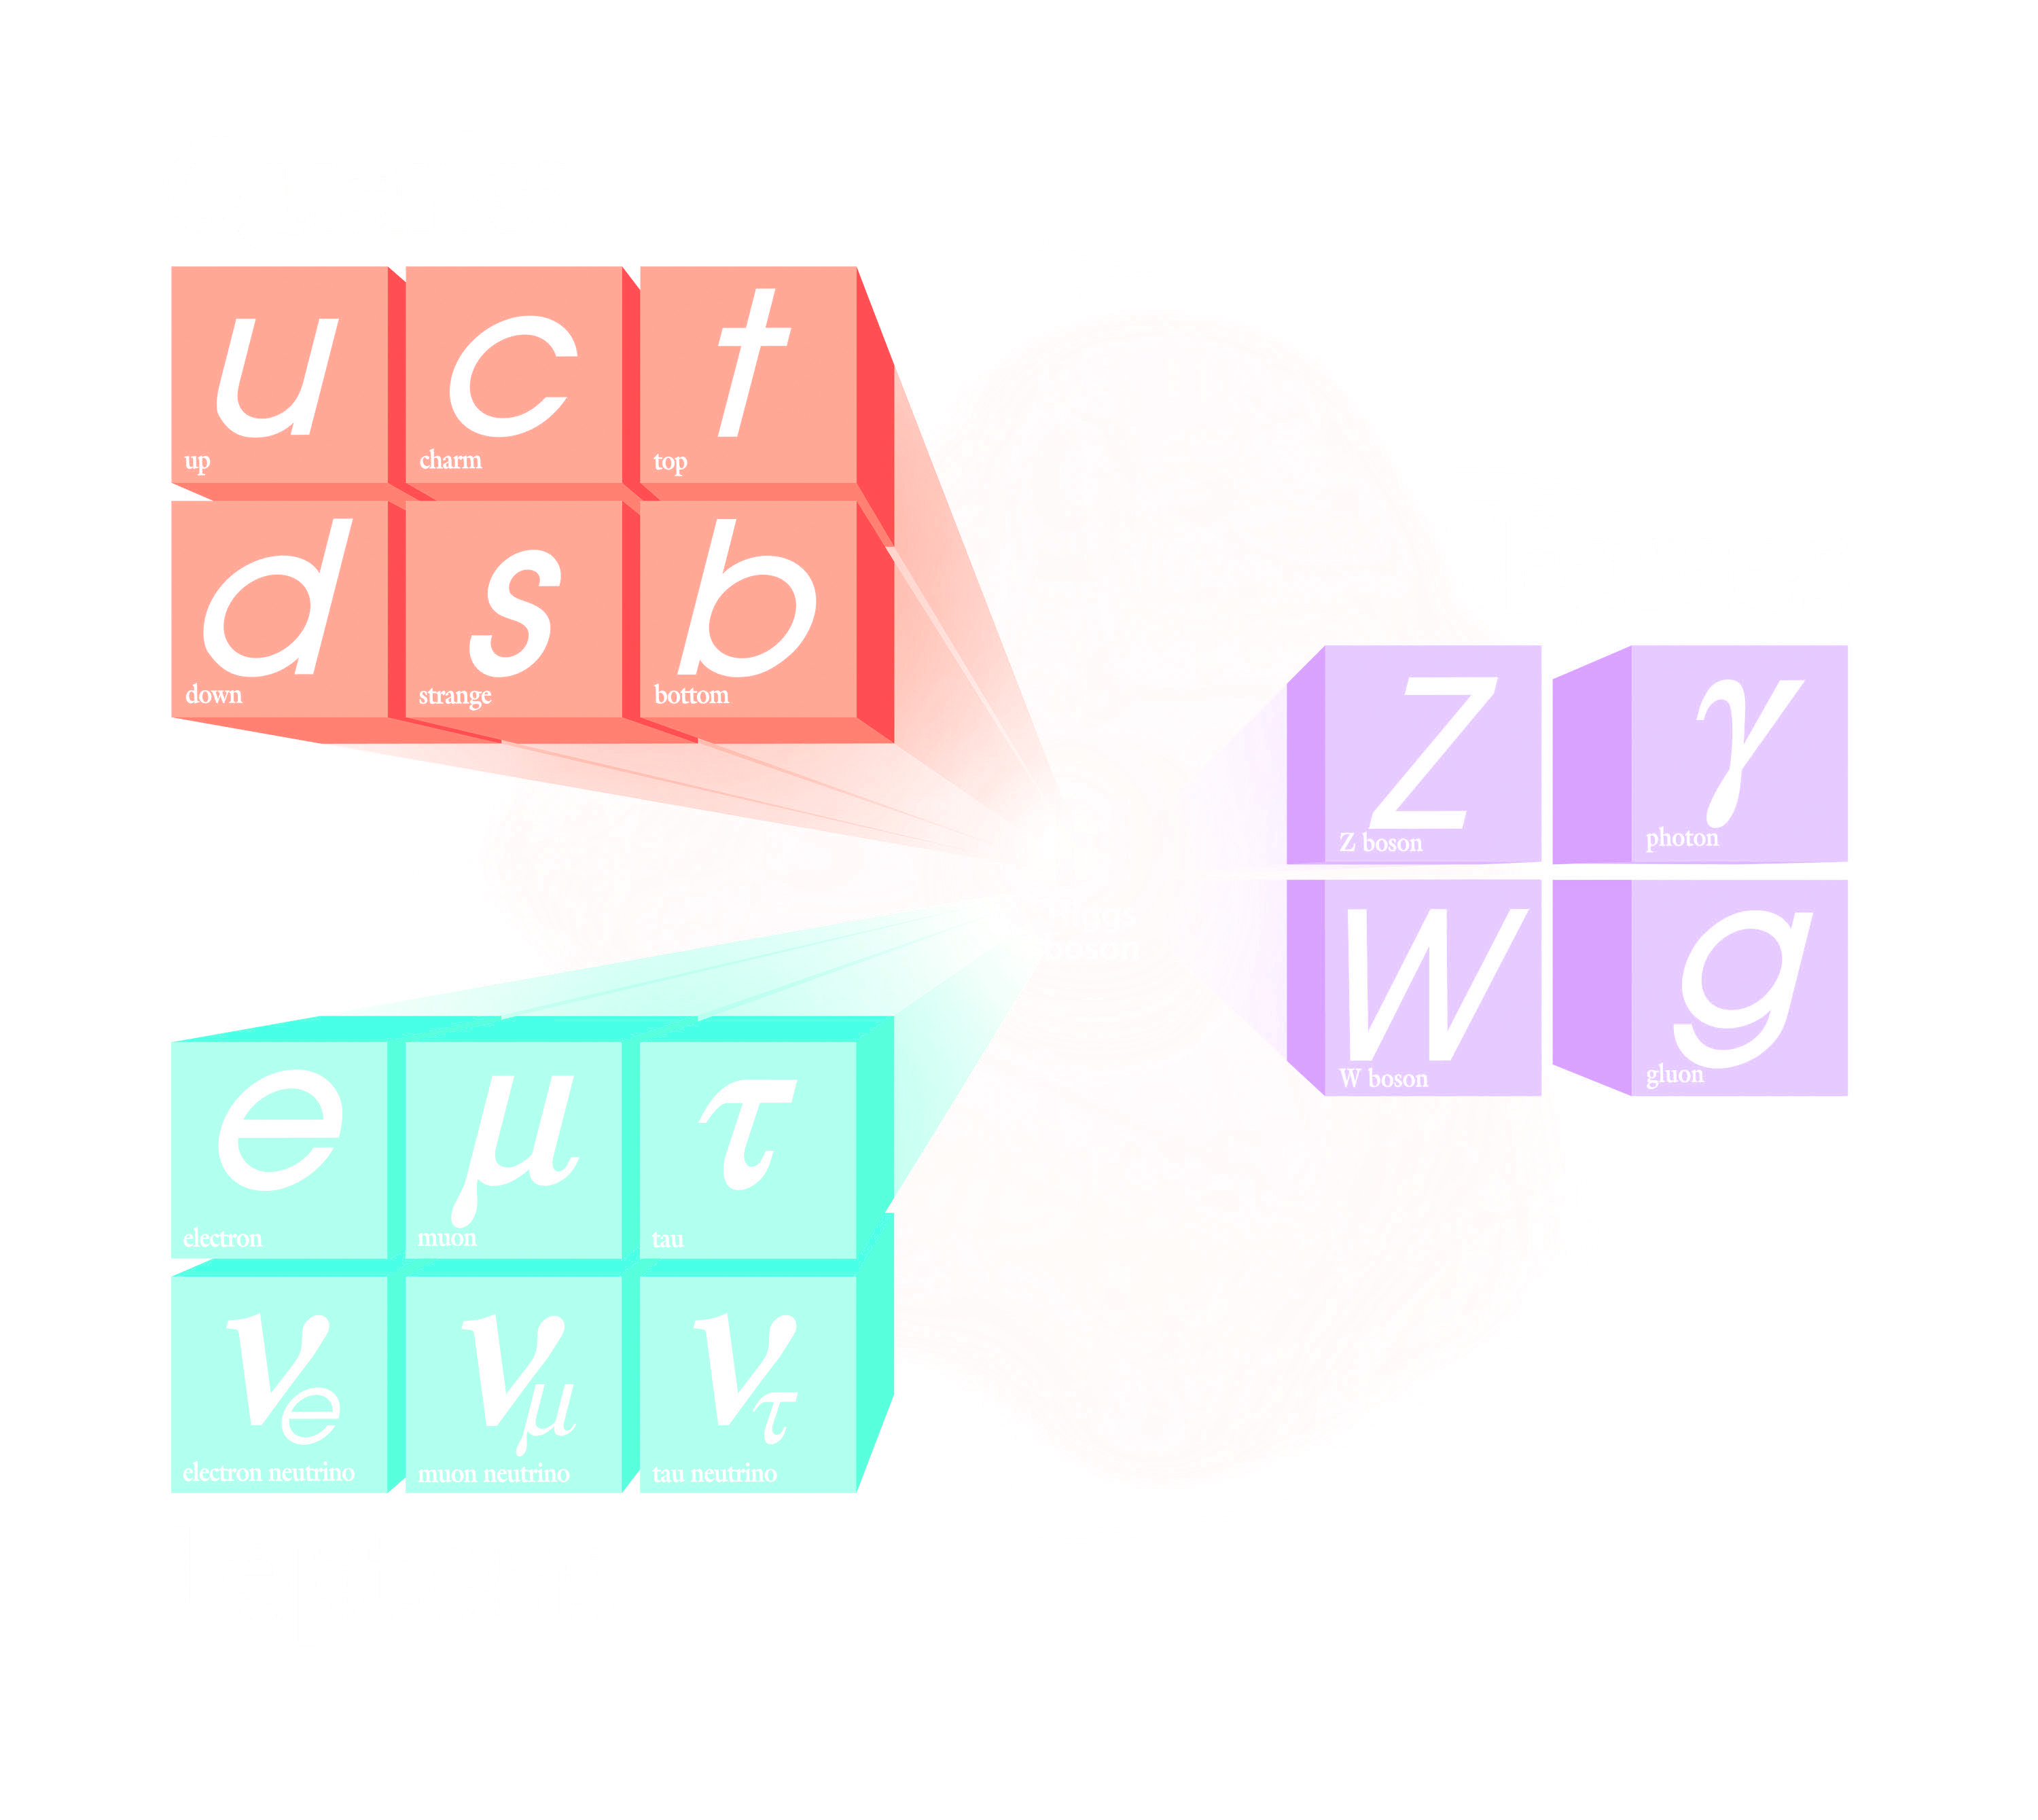
\includegraphics[width=15cm,trim=25 25 25 25,clip]{{general/particles}.png}         
           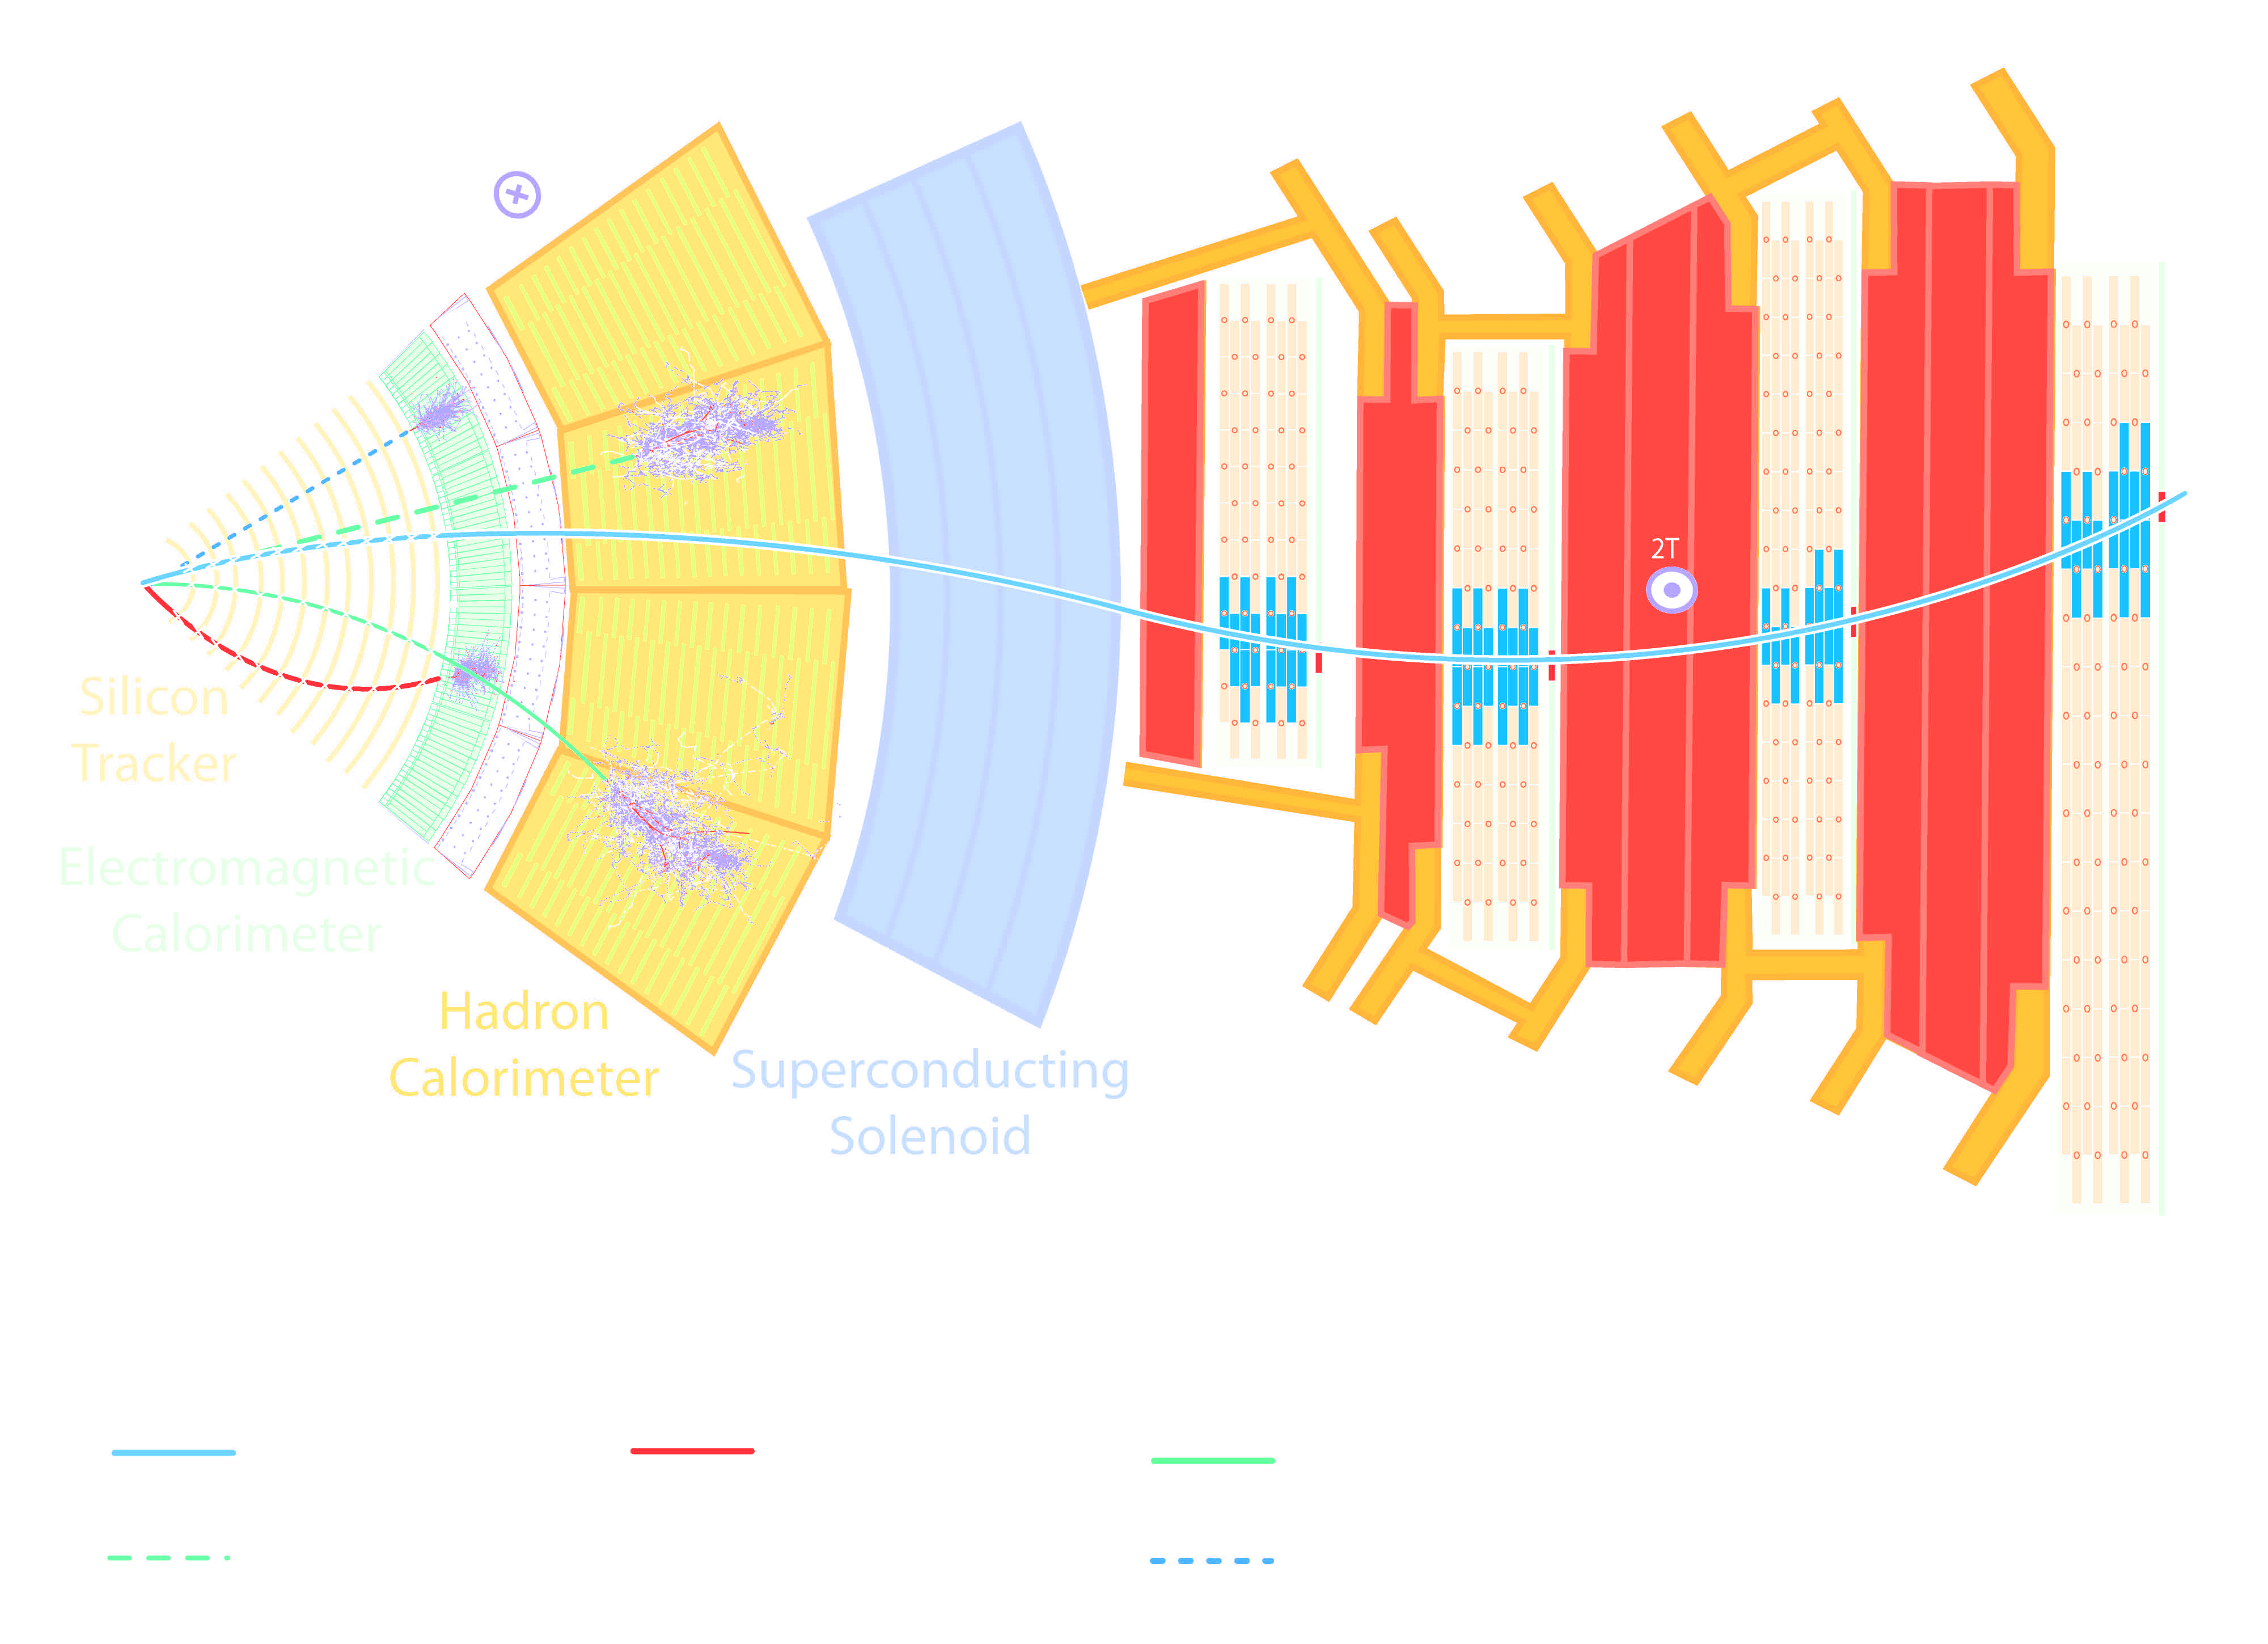
\includegraphics[width=15cm,trim=25 25 25 25,clip]{{general/pf}.png}           
          \end{figure}
          \color{white}
          \small
         Multiple observations and the everyday experience of gravity hint at the fact that the Standard Model (SM) is not the ultimate theory of nature. Why is the Higgs boson so light? Why is matter so abundant compared to antimatter? Why is gravity so much weaker than the other forces? How can neutrinos be so light?
New data, never before explored, might hold keys to unlocking these secrets about the fundamental nature of nature itself! Data collected in the recently finished Run II, at the never aforetime reached energy of 13 TeV, will provide a matchless opportunity for joining this expedition into the high energy frontier. There are several available thesis subjects focussed on analysing the many uncharted dwellings in the LHC's data, all complementary to the research being performed in the Gent CMS group.
       \end{minipage}

    };
 %   \node[fancytitle, left=\titleOffset] at (ugentBox.north east) {Data analysis at CMS};

